\documentclass{capstonedoc}

% Document Info
\title{Sega Genesis Controller Interfacing}
\date{2016-03-13}
\author{Mason Strong, Stephen Just}

\usepackage{cite}
\usepackage[hyphens]{url}

\usepackage{wrapfig}
\usepackage{graphicx}
\graphicspath{ {images/} }

\usepackage{caption}

\begin{document}
\maketitle

%Document body

\begin{wrapfigure}{r}{0.4\textwidth}
  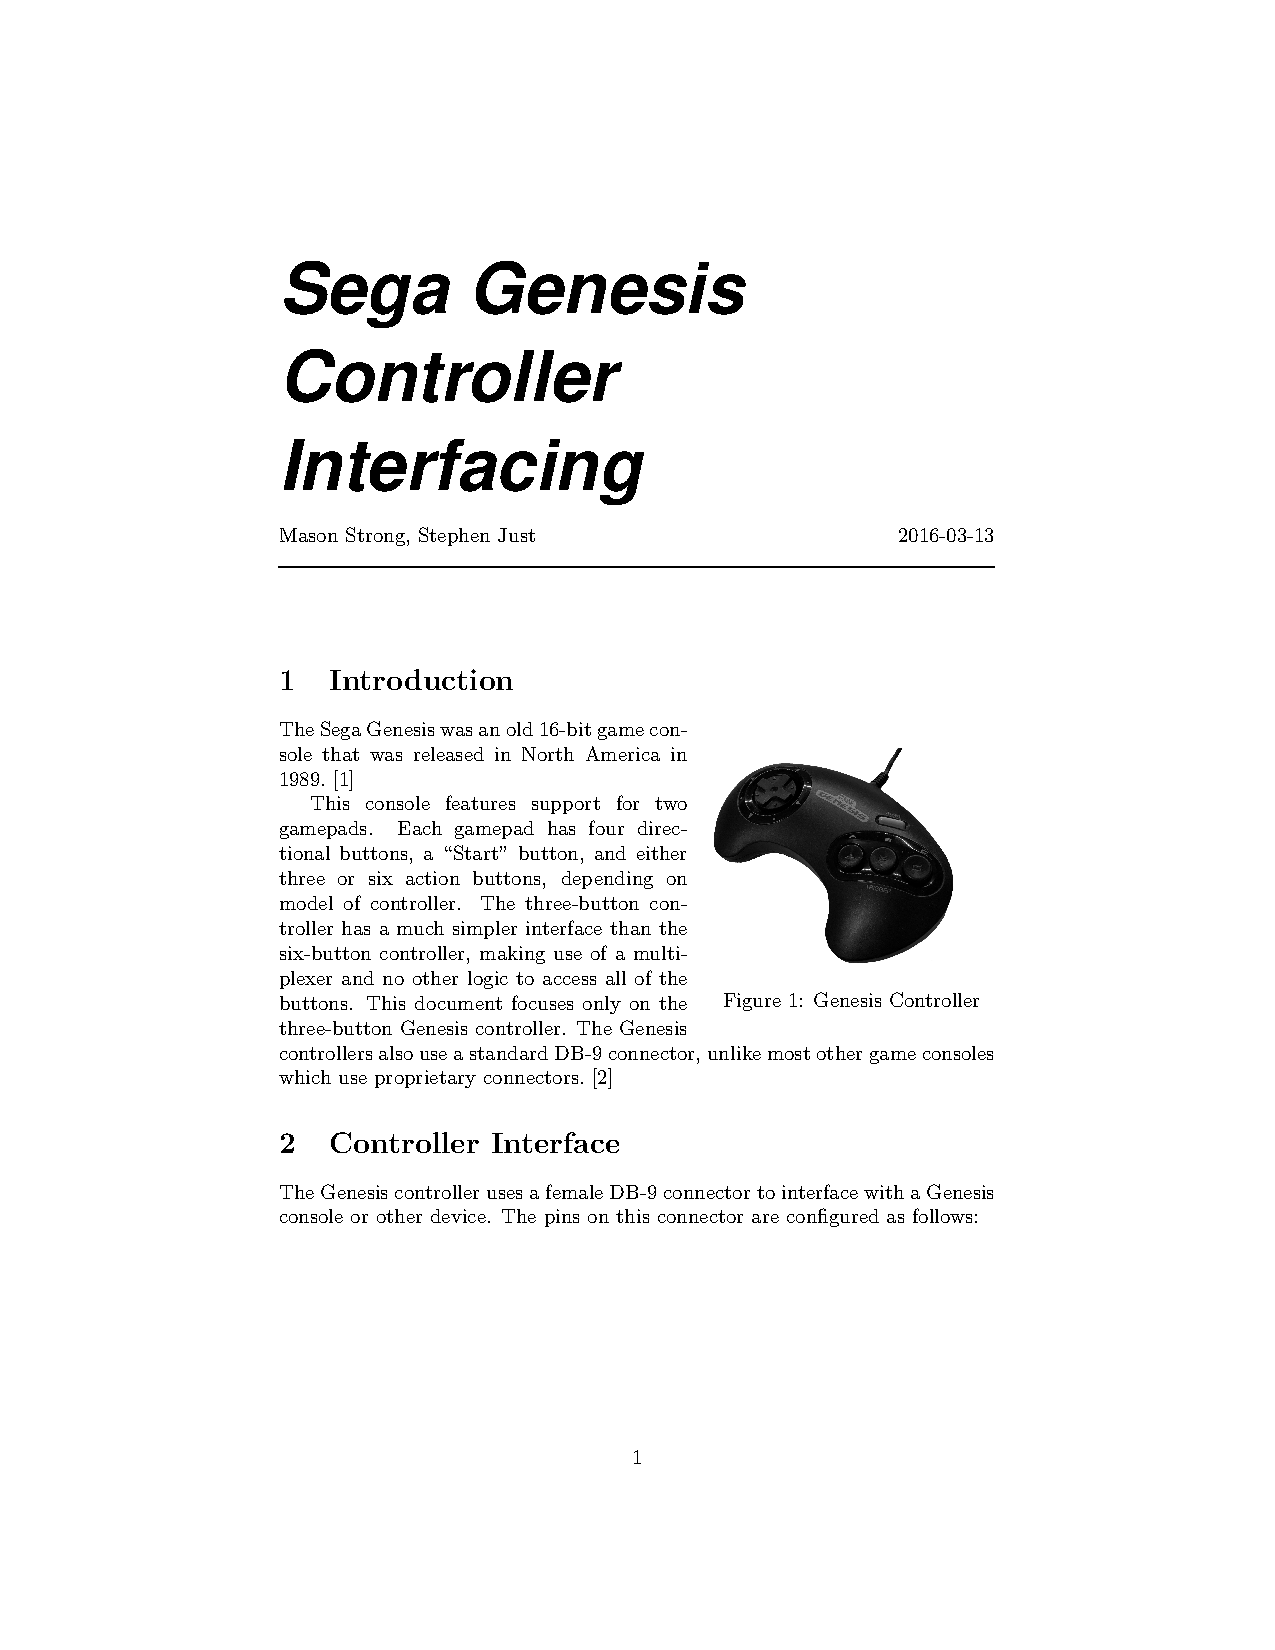
\includegraphics[width=0.35\textwidth]{genesis_controller}
  \caption{Genesis Controller}
  \label{fig:controller_photo}
\end{wrapfigure}

\section{Introduction}
The Sega Genesis was an old 16-bit game console that was released in North
America in 1989. \cite{SGHistory}

This console features support for two gamepads. Each gamepad has four
directional buttons, a ``Start'' button, and either three or six action
buttons, depending on model of controller. The three-button controller has a
much simpler interface than the six-button controller, making use of a
multiplexer and no other logic to access all of the buttons. This document
focuses only on the three-button Genesis controller. The Genesis controllers
also use a standard DB-9 connector, unlike most other game consoles which
use proprietary connectors.\cite{SGCHwInfo}

\section{Controller Interface}
The Genesis controller uses a female DB-9 connector to interface with a Genesis
console or other device. The pins on this connector are configured as follows:

\vspace{5mm}
\begin{tabular}{ l | l | l }
  Pin & Func (select low) & Func (select high) \\ \hline \hline
  1   & up button         & up button          \\
  2   & down button       & down button        \\
  3   & logic low         & left button        \\
  4   & logic low         & right button       \\
  5   & Power (+5 volts)  & Power (+5 Volts)   \\
  6   & A button          & B button           \\
  7   & select signal     & select signal      \\
  8   & Ground            & Ground             \\
  9   & Start button      & C button           \\
\end{tabular}
\vspace{5mm}

While the controller was designed for +5 Volts for power, because of its simple
design, it is possible to determine that it is actually capable of 2 - 6 Volts.
This is possible because the controller only contains a single 74HC157
multiplexer chip inside, whose datasheet specifies that the device is operable
within that range, with varying delay times.\cite{TC74HC157AP}

In order to read the buttons on a controller, the master device should apply
a logic high or low to the select pin of the controller, and then query the
state of each of the button pins. Then the master device can switch the state
of the select pin, and then query the values for the other buttons. When a
button is pressed, its value will be logic low. Buttons that are not pressed
will appear as a logic high. Note that reading the up and down buttons of
the controller are not affected by the select signal, as they are connected
directly to the controller plug and not through the multiplexer.

\section{Notes}
On a real Genesis console, the controller's value is read once per video frame,
or 60 times per second. That means that if you are trying to emulate a
controller, the emulated buttons should remain pressed for at least 1/60th of
a second, to ensure that the input is received by the console. Shorter button
presses could be missed entirely.

Be aware that the six-button gamepad has a more complicated interface protocol.
The extra buttons are accessed by toggling the select line on the controller
three times in quick succession. If you want your application to tolerate six-
button controllers, take care not to do this. The six-button controllers should
not go in to this mode if you only toggle the select line once per frame.
This appnote targets the standard three-button genesis controllers and 
corresponding protocol.

\section{Project Setup}
Ensure that you are in possession of a three-button genesis controller, and a 
corresponding adapter board to interface the DB9 connector with the appropriate 
GPIO pins on the DE2. Should an adapter board be unavailable, a 40-pin ribbon 
cable breadboarded with a male DB9 connector according to the pinout described 
in Figure~\ref{fig:schematic}.

\begin{figure}[h]
  \centering
  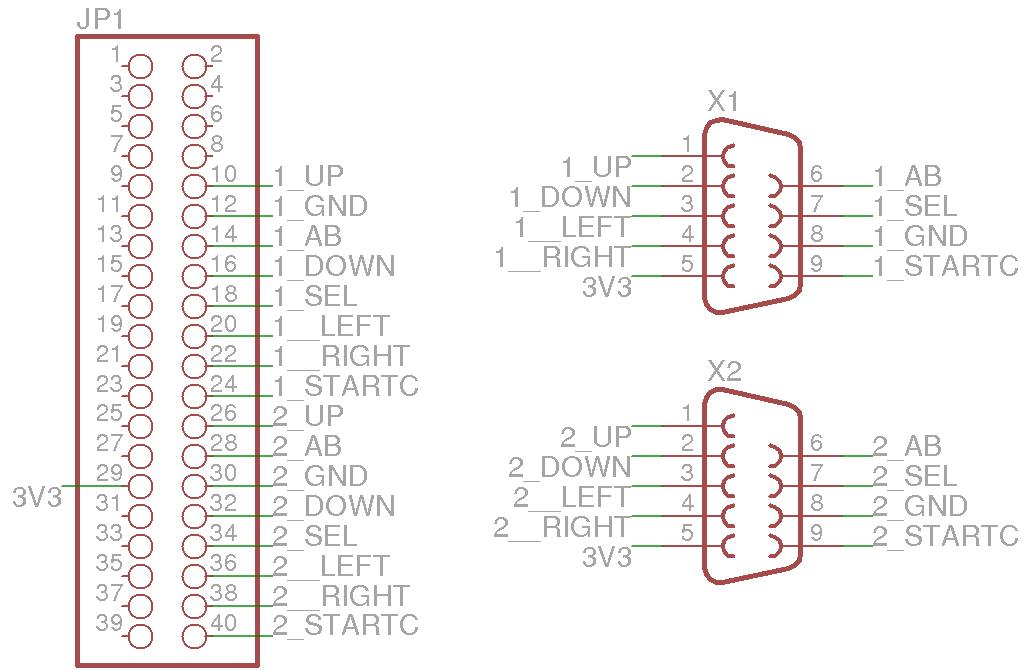
\includegraphics[width=7cm]{schematic}
  \caption{Connection Schematic}
  \label{fig:schematic}
\end{figure}

In a typical video game system, you might want to trigger the Genesis controller
from a 60Hz pulse, such as a video VSync signal. However, to simplify this demo,
there is a simple process in the VHDL top-level file to generate a pulse
every 50ms to trigger the Genesis controller block.

\subsection{Qsys}

In order to use a genesis controller, a custom component must be created in
Qsys. This component is provided in the companion code to this application note,
found in the \texttt{ip} directory. The following instructions detail how you
might recreate this block, and set up a Qsys system to use it. The provided demo
system is set up slightly differently, to use LEDs as an output.

\begin{enumerate}
  \item Name the component \texttt{genesis}
  \item Provide \texttt{custom\_controller.vhd} as the synthesis file
  \item Setup the signals as shown below in figure~\ref{fig:qsys_signals}:

    \begin{figure}[h]
      \centering
      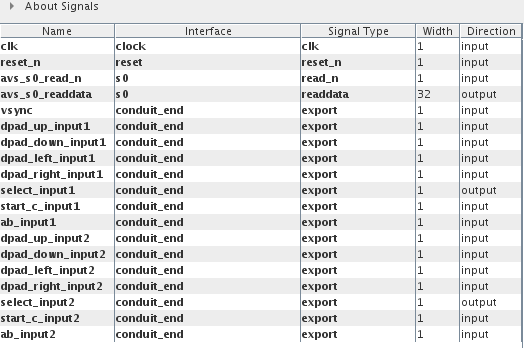
\includegraphics[width=7cm]{fig1}
      \caption{Genesis Component Signals}
      \label{fig:qsys_signals}
    \end{figure}

  \item Configure the component interfaces as in figures
    \ref{fig:qsys_signals2}, \ref{fig:qsys_signals3}, and
    \ref{fig:qsys_signals4}:

    \begin{figure}[h!]
      \centering
      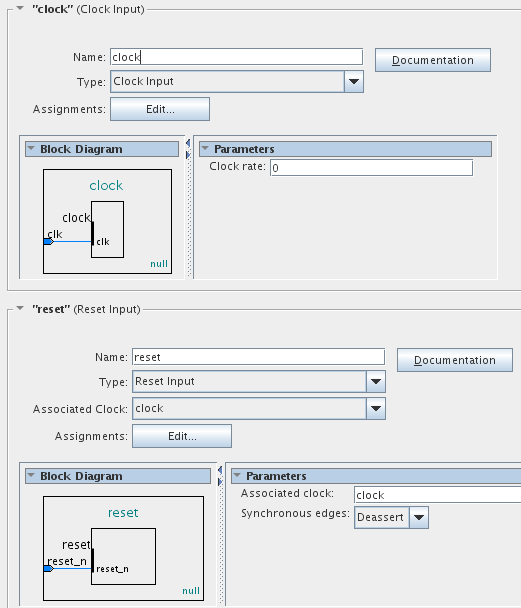
\includegraphics[width=10cm]{fig2}
      \caption{Genesis Component Clock and Reset Configuration}
      \label{fig:qsys_signals2}
    \end{figure}

    \begin{figure}[h!]
      \centering
      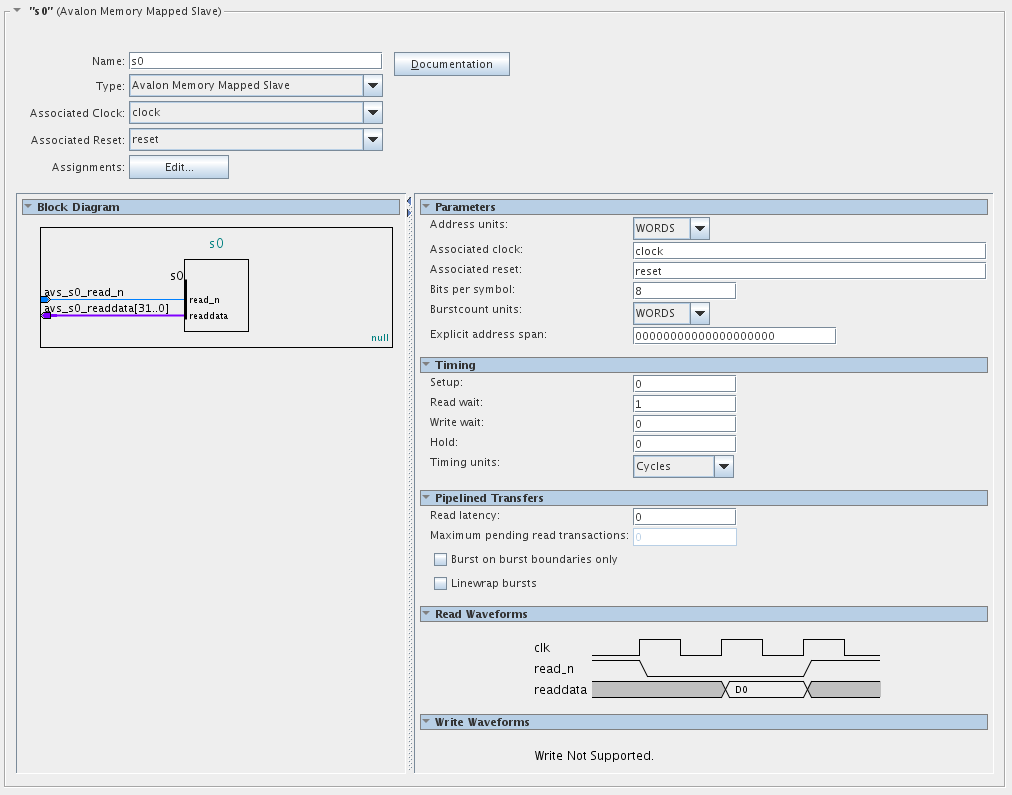
\includegraphics[width=10cm]{fig3}
      \caption{Genesis Component MM Slave Configuration}
      \label{fig:qsys_signals3}
    \end{figure}

    \begin{figure}[h!]
      \centering
      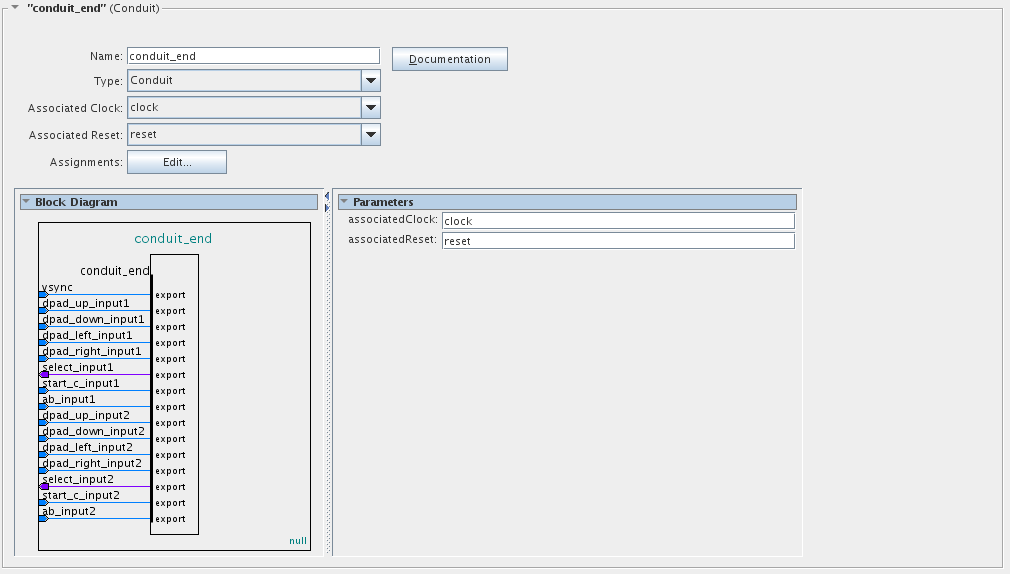
\includegraphics[width=10cm]{fig4}
      \caption{Genesis Component Conduit Configuration}
      \label{fig:qsys_signals4}
    \end{figure}

  \item Add the custom component to your system. Connect \texttt{clock},
    \texttt{s0}, and \texttt{reset} appropriately.
    Ensure that \texttt{conduit\_end} is exported properly. An example of this
    configuration is shown in figure~\ref{fig:qsys_signals5}.

    \begin{figure}[h]
      \centering
      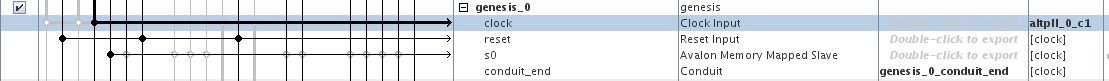
\includegraphics[width=10cm]{fig5}
      \caption{Genesis Component Qsys Connections}
      \label{fig:qsys_signals5}
    \end{figure}


  \item Regenerate base addresses in the event of conflicts.

\end{enumerate}

\subsection{Quartus}

The Genesis controllers are connected to the DE2 via one of the GPIO ports. In
our system, we used \texttt{GPIO\_1}. To ensure correct controller behaviour,
the GPIO connector should be configured as high-impedance by default, as is
shown in Listing~\ref{lst:tl_port}.

\begin{lstlisting}[language={vhdl},caption={Entity Port for Genesis Controllers},label={lst:tl_port}]
  VGA_VS : buffer std_logic;
  GPIO_1 : inout std_logic_vector (35 downto 0) := (others => 'Z');
\end{lstlisting}

The Qsys system containing the Genesis controller interface component includes
the ports similar to the ones shown in Listing~\ref{lst:comp_port} within its
component declaration.

\begin{lstlisting}[language={vhdl},caption={Qsys System Ports for Genesis Controller},label={lst:comp_port}]
  genesis_0_conduit_end_vsync  : in    std_logic  := 'X';             -- trigger signal, usually vsync
  genesis_0_conduit_end_dpad_up_input1            : in    std_logic  := 'X';             -- dpad_up_input1
  genesis_0_conduit_end_dpad_down_input1          : in    std_logic  := 'X';             -- dpad_down_input1
  genesis_0_conduit_end_dpad_left_input1          : in    std_logic  := 'X';             -- dpad_left_input1
  genesis_0_conduit_end_dpad_right_input1         : in    std_logic  := 'X';             -- dpad_right_input1
  genesis_0_conduit_end_select_input1             : out   std_logic;                     -- select_input1
  genesis_0_conduit_end_start_c_input1            : in    std_logic  := 'X';             -- start_c_input1
  genesis_0_conduit_end_ab_input1                 : in    std_logic  := 'X';             -- ab_input1
  genesis_0_conduit_end_dpad_up_input2            : in    std_logic  := 'X';             -- dpad_up_input2
  genesis_0_conduit_end_dpad_down_input2          : in    std_logic  := 'X';             -- dpad_down_input2
  genesis_0_conduit_end_dpad_left_input2          : in    std_logic  := 'X';             -- dpad_left_input2
  genesis_0_conduit_end_dpad_right_input2         : in    std_logic  := 'X';             -- dpad_right_input2
  genesis_0_conduit_end_select_input2             : out   std_logic;                     -- select_input2
  genesis_0_conduit_end_start_c_input2            : in    std_logic  := 'X';             -- start_c_input2
  genesis_0_conduit_end_ab_input2                 : in    std_logic  := 'X';             -- ab_input2
\end{lstlisting}

The instance of the Qsys system defines which pins on the DE2's GPIO header are
connected to the pins on the Genesis controllers. The configuration used for our
interface PCB is shown in Listing~\ref{lst:port_map}.

\begin{lstlisting}[language={vhdl},caption={Port Map Configuration},label={lst:port_map}]
  video_vga_controller_0_external_interface_VS => VGA_VS,
  genesis_0_conduit_end_vsync  => genesis_trigger,
  genesis_0_conduit_end_dpad_up_input1            => GPIO_1(9),
  genesis_0_conduit_end_dpad_down_input1          => GPIO_1(13),
  genesis_0_conduit_end_dpad_left_input1          => GPIO_1(17),
  genesis_0_conduit_end_dpad_right_input1         => GPIO_1(19),
  genesis_0_conduit_end_select_input1             => GPIO_1(15),
  genesis_0_conduit_end_start_c_input1            => GPIO_1(21),
  genesis_0_conduit_end_ab_input1                 => GPIO_1(11),
  genesis_0_conduit_end_dpad_up_input2            => GPIO_1(23),
  genesis_0_conduit_end_dpad_down_input2          => GPIO_1(27),
  genesis_0_conduit_end_dpad_left_input2          => GPIO_1(31),
  genesis_0_conduit_end_dpad_right_input2         => GPIO_1(33),
  genesis_0_conduit_end_select_input2             => GPIO_1(29),
  genesis_0_conduit_end_start_c_input2            => GPIO_1(35),
  genesis_0_conduit_end_ab_input2                 => GPIO_1(25),
\end{lstlisting}

Compile the project to ensure it is working. 

\subsection{Eclipse}

A sample workspace is included in the companion code to read the Genesis
controllers connected to the system, and output to the red LEDs on the DE2.
This is located in the \texttt{software} directory of the companion code
package.

\section{Reading from the Controllers}

The current state for each button for either controller is stored 
in a 32-bit value, with 16 of those bits corresponding to a button 
on either controller. By reading the memory at \texttt{GENESIS\_0\_BASE}, 
one can examine a particular bit to determine which button is being 
pressed. The code below illustrates this simply: 

\begin{lstlisting}[language={c},tabsize=2,caption={Reading Genesis Controller State}]
	  int genesis_value = IORD_32DIRECT(GENESIS_0_BASE, 0);

	  if ((genesis_value)& (1 << 0)){
		  printf("1 Up was pressed\n");
	  }
	  if ((genesis_value)& (1 << 1)){
		  printf("1 Down was pressed\n");
	  }
	  if ((genesis_value)& (1 << 2)){
		  printf("1 Left was pressed\n");
	  }
	  if ((genesis_value)& (1 << 3)){
		  printf("1 Right was pressed\n");
	  }
	  if ((genesis_value)& (1 << 4)){
		  printf("1 A was pressed\n");
	  }
	  if ((genesis_value)& (1 << 5)){
		  printf("1 B was pressed\n");
	  }
	  if ((genesis_value)& (1 << 6)){
		  printf("1 C was pressed\n");
	  }
	  if ((genesis_value)& (1 << 7)){
		  printf("1 Start was pressed\n");
	  }

	  if ((genesis_value)& (1 << 10)){
		  printf("2 Up was pressed\n");
	  }
	  if ((genesis_value)& (1 << 11)){
		  printf("2 Down was pressed\n");
	  }
	  if ((genesis_value)& (1 << 12)){
		  printf("2 Left was pressed\n");
	  }
	  if ((genesis_value)& (1 << 13)){
		  printf("2 Right was pressed\n");
	  }
	  if ((genesis_value)& (1 << 14)){
		  printf("2 A was pressed\n");
	  }
	  if ((genesis_value)& (1 << 15)){
		  printf("2 B was pressed\n");
	  }
	  if ((genesis_value)& (1 << 16)){
		  printf("2 C was pressed\n");
	  }
	  if ((genesis_value)& (1 << 17)){
		  printf("2 Start was pressed\n");
	  }
\end{lstlisting}

\newpage

% References
\bibliographystyle{ieeetr}
\bibliography{genesis_controller}

\end{document}
